\documentclass[12pt]{article}
\usepackage{color}
\usepackage{multicol,ifthen,booktabs,amsmath,amsfonts,bm,mathrsfs,amssymb}
\usepackage{times,mathptmx}
\usepackage{braket}
\usepackage{enumerate}
\usepackage{geometry}
\usepackage{graphicx}% Include figure files
\usepackage{listings}
\usepackage[latin1]{inputenc}
\usepackage{tikz}
\usepackage{tikz-feynman}
\usetikzlibrary{trees}
\usetikzlibrary{decorations.pathmorphing}
\usetikzlibrary{decorations.markings}
\usepackage{verbatim}
\renewcommand\baselinestretch{1.5}\protect
\abovedisplayshortskip 3 pt
\belowdisplayshortskip 3 pt
\geometry{left=2cm,right=2cm,top=3cm,bottom=3cm}
\graphicspath{{./figures/}{./}}

% Define styles for the different kind of edges in a Feynman diagram
\tikzset{
    fermion/.style={draw=black, postaction={decorate},
        decoration={markings,mark=at position .55 with {\arrow[draw=black]{>}}}},
    fermionbar/.style={draw=black, postaction={decorate},
        decoration={markings,mark=at position .55 with {\arrow[draw=black]{<}}}},
    fermionnoarrow/.style={draw=black},
    gluon/.style={decorate, draw=orange,
        decoration={coil,amplitude=3pt, segment length=4pt}},
    scalar/.style={dashed,draw=red},
    scalarpi/.style={dashed,draw=blue},
}

\begin{document}

\section{Flow equation}
\begin{eqnarray}
\begin{split}
\partial_t \Gamma_k  \sim & \partial_t \{\bar q  m_f q \} \\
= &- \tilde{\partial_t}
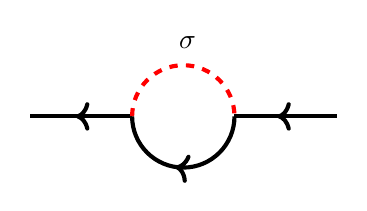
\begin{tikzpicture}[line width=1.5 pt, scale=1.3]
	\draw[fermion] (0:1)--(0,0);
	\draw[scalar] (1,0) arc (180:0:.5);
          \draw[fermion] (2,0) arc (0:-180:.5);
	\draw[fermionbar] (2,0) --(3,0);
          \node  at (25:1.7) {$\sigma$};
\end{tikzpicture}\\
&- \tilde{\partial_t}
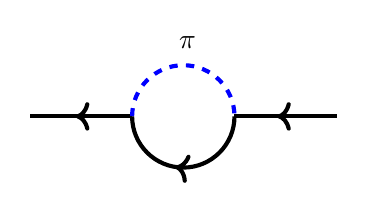
\begin{tikzpicture}[line width=1.5 pt, scale=1.3]
	\draw[fermion] (0:1)--(0,0);
	\draw[scalarpi] (1,0) arc (180:0:.5);
	\draw[fermion] (2,0) arc (0:-180:.5);
	\draw[fermionbar] (2,0) --(3,0);
          \node  at (25:1.7) {$\pi$};
\end{tikzpicture}\\
&- \tilde{\partial_t}
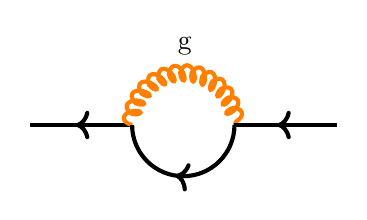
\begin{tikzpicture}[line width=1.5 pt, scale=1.3]
	\draw[fermion] (0:1)--(0,0);
	\draw[gluon] (1,0) arc (180:0:.5);
	\draw[fermion] (2,0) arc (0:-180:.5);
          \node  at (27:1.7) {g};
	\draw[fermionbar] (2,0) --(3,0);
\end{tikzpicture}
\end{split}
\end{eqnarray}
\begin{eqnarray}
\begin{split}
\partial_t (m_f(p))^\sigma=&
- \tilde{\partial_t} \Bigg ( \frac{1}{4} tr \Bigg (
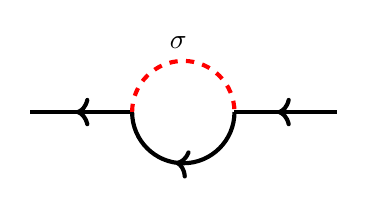
\begin{tikzpicture}[line width=1.5 pt, scale=1.3]
	\draw[fermion] (0:1)--(0,0);
	\draw[scalar] (1,0) arc (180:0:.5);
          \draw[fermion] (2,0) arc (0:-180:.5);
	\draw[fermionbar] (2,0) --(3,0);
          \node  at (25:1.6) {$\sigma$};
\end{tikzpicture}
\Bigg )\Bigg |_p \Bigg )\\
=& - \tilde{\partial_t}\sum \!\!\!\!\!\!\!\!\!\int \Bigg ( \frac{1}{Z_{\phi,k} Z_{q,k}}\frac{h^2_k}{4} \bar m_f \bar G^q_k (q) \bar G^{\sigma}_k(q-p) \Bigg )\\
=&- \frac{1}{Z_{\phi,k} Z_{q,k}}\frac{h^2_k}{4} \bar m_f \sum \!\!\!\!\!\!\!\!\!\int  \bigg (  \tilde{\partial_t}  \bar G^q_k (q) \bar G^{\sigma}_k(q-p)+\bar G^q_k (q-p) \tilde{\partial_t}  \bar G^{\sigma}_k(q) \bigg )
\end{split}
\end{eqnarray}
\begin{eqnarray}
\tilde{\partial_t}  \bar G^q_k (q) = -2k^2 (\bar G^q_k(q))^2 [(1-\eta_q)+\eta_q x^{\frac{1}{2}}]\theta(1-x)
\end{eqnarray}
\begin{eqnarray}
\tilde{\partial_t}  \bar G^{\sigma}_k (q) = -k^2 (\bar G^{\sigma}_k(q))^2 [(2-\eta_\phi)+\eta_\phi x]\theta(1-x)
\end{eqnarray}
\begin{eqnarray}
\begin{split}
&T \sum_n\int \frac{d^3q}{(2 \pi)^3}(\tilde{\partial_t}  \bar G^q_k (q)) \bar G^{\sigma}_k(q-p)\\
=&T \sum_n \int \frac{d^3q}{(2 \pi)^3} (-2)\frac{1}{k^2} (\tilde G^q_k(q))^2 [(1-\eta_q)+\eta_q x^{\frac{1}{2}}]\theta(1-x)\frac{1}{k^2} \tilde G^{\sigma}_k(q-p) \\
=& -\frac{2}{k^4} \frac{1}{(2\pi)^3}\int_0^{\infty} q^2 dq \int_{-1}^{1} d \cos \theta  (2\pi)[(1-\eta_q)+\eta_q x^{\frac{1}{2}}]\theta(1-x) T \sum_n \tilde G^q_k(q))^2 \tilde G^{\sigma}_k(q-p) \\
=&-\frac{1}{(2 \pi)^2} \int_{0}^{1}  x^{\frac{1}{2}}[(1-\eta_q)+\eta_q x^{\frac{1}{2}}] dx \int_{-1}^{1} d \cos \theta \frac{T}{k} \sum_n \tilde G^q_k(q))^2 \tilde G^{\sigma}_k(q-p) 
\end{split}
\end{eqnarray}
here we note that
\begin{eqnarray}
\begin{split}
\mathcal{F}2\mathcal{B}1p(m_q;m_{\phi})&\equiv \frac{T}{k} \sum_n \tilde G^q_k(q))^2 \tilde G^{\phi}_k(q-p) \\
&=\mathcal{F}2\mathcal{B}1(m_q;m_{\phi,q-p})
\end{split}
\end{eqnarray}
Then
\begin{eqnarray}
above=-\frac{1}{(2 \pi)^2} \int_{0}^{1}  x^{\frac{1}{2}}[(1-\eta_q)+\eta_q x^{\frac{1}{2}}] dx \int_{-1}^{1} d \cos \theta \mathcal{F}2\mathcal{B}1(m_q;m_{\sigma,q-p})
\end{eqnarray}
\begin{eqnarray}
\begin{split}
&T \sum_n\int \frac{d^3q}{(2 \pi)^3}\bar G^q_k (q-p)\tilde{\partial_t}  \bar G^{\sigma}_k(q)\\
&=-\frac{1}{2(2 \pi)^2}\int_0^1 x^{\frac{1}{2}}[(2-\eta_\phi)+\eta_\phi x] dx\int_{-1}^{1} d\cos \theta \mathcal{F}1\mathcal{B}2(m_{q,q-p};m_{\sigma})
\end{split}
\end{eqnarray}
Then
\begin{eqnarray}
\begin{split}
\partial_t (\bar m_f(p))^\sigma=&\frac{\bar h_k^2 \bar m_{f,k}}{8 (2 \pi)^2}\bigg (2 \int_{0}^{1}  x^{\frac{1}{2}}[(1-\eta_q)+\eta_q x^{\frac{1}{2}}] dx \int_{-1}^{1} d \cos \theta \mathcal{F}2\mathcal{B}1(m_q;m_{\sigma,q-p})\\
&+\int_0^1 x^{\frac{1}{2}}[(2-\eta_\phi)+\eta_\phi x] dx\int_{-1}^{1} d\cos \theta \mathcal{F}1\mathcal{B}2(m_{q,q-p};m_{\sigma}) \bigg )
\end{split}
\end{eqnarray}
similar
\begin{eqnarray}
\begin{split}
\partial_t (\bar m_f(p))^\pi=&\frac{3\bar h_k^2 \bar m_{f,k}}{8 (2 \pi)^2}\bigg (2 \int_{0}^{1}  x^{\frac{1}{2}}[(1-\eta_q)+\eta_q x^{\frac{1}{2}}] dx \int_{-1}^{1} d \cos \theta \mathcal{F}2\mathcal{B}1(m_q;m_{\pi,q-p})\\
&+\int_0^1 x^{\frac{1}{2}}[(2-\eta_\phi)+\eta_\phi x] dx\int_{-1}^{1} d\cos \theta \mathcal{F}1\mathcal{B}2(m_{q,q-p};m_{\pi}) \bigg )
\end{split}
\end{eqnarray}
\begin{eqnarray}
\begin{split}
\partial_t (\bar m_f(p))^A=&-\frac{3\bar m_{f,k} \bar{g}^2_kC_2(N_c)}{2 (2 \pi)^2}\bigg (2 \int_{0}^{1}  x^{\frac{1}{2}}[(1-\eta_q)+\eta_q x^{\frac{1}{2}}] dx \int_{-1}^{1} d \cos \theta \mathcal{F}2\mathcal{B}1(m_q;m_{A,q-p})\\
&+\int_0^1 x^{\frac{1}{2}}[(2-\eta_A)+\eta_A x] dx\int_{-1}^{1} d\cos \theta \mathcal{F}1\mathcal{B}2(m_{q,q-p};m_{A}) \bigg )
\end{split}
\end{eqnarray}
\begin{eqnarray}
\partial_t (\bar m_f(p))=\partial_t (\bar m_f(p))^\sigma+\partial_t (\bar m_f(p))^\pi+\partial_t (\bar m_f(p))^A
\end{eqnarray}
\begin{eqnarray}
\begin{split}
\bar m_f(p)&=\bar m_f(p)\Big|_\Lambda+\int_0^{ln(IR/\Lambda)}(\partial_t (\bar m_f(p)) dt=0+\int_\Lambda^{IR}(\partial_t (\bar m_f(p)) \frac{dk}{k}\\
&=-\int_{IR}^{\Lambda}\frac{\partial_t (\bar m_f(p)} {k}dk
\end{split}
\end{eqnarray}
\end{document}
